\section{Аналитическая часть}

В данном разделе будут проанализированы существующие решения, а также рассмотрена архитектура СУБД ClickHouse и движка MergeTree.

\subsection{Базовые понятия}

В данном подразделе будут рассмотрены базовые понятия, необходимые для понимания устройства существующих решений.

\subsubsection{Хэш-функция}

Хэш-функция\cite{hash} --- функция, осуществляющая преобразование массива входных данных произвольной длины в выходную битовую строку установленной длины, выполняемое определённым алгоритмом.

Хэш-функции применяются:
\begin{itemize}
    \item[---] при решении задачи дедубликации;
    \item[---] при построении идентификаторов;
    \item[---] при вычислении контрольных сумм;
    \item[---] при хранении паролей.
\end{itemize}

Криптографическая стойкость \cite{crypto} --- способность криптографического алгоритма противостоять криптоанализу. Стойким считается алгоритм, успешная атака на который требует от атакующего обладания недостижимым на практике объёмом вычислительных ресурсов либо настолько значительных затрат времени на раскрытие, что к его моменту защищённая информация утратит свою актуальность.

При рассмотрении хэш-функций под алгоритмом подразумевается процесс вычисления значения хэш-функции, а под атакой на алгоритм --- решение обратной задачи: нахождение для заданного значения хэш-функции \textit{H1} такого массива входных данных \textit{A1}, что \textit{f(A1) = H1}. Хэш-функцию, которая является стойкой по определению криптографической стойкости по отношению к такой задаче, называют криптостойкой.

Криптостойкие функции также обладают следующим свойством: при наличии массива входных данных \textit{A1} и значения хэш-функции для него \textit{f(A1)}, настолько же сложной задачей, что и нахождения обратного значения, является задача нахождения такого отличного от \textit{A1} значения массива входных данных \textit{A2}, для которого верно \textit{f(A1) = f(A2)}. Такие значения \textit{A1} и \textit{A2}, для которых верно равенство \textit{f(A1) = f(A2)}, называются коллизиями.

\subsubsection{Блокчейн}

Блокчейн\cite{bitcoin} --- выстроенная по определённым правилам непрерывная последовательная цепочка блоков --- элементов, содержащих информацию. В общем случае такая цепочка поддерживает 2 операции:
\begin{enumerate}
    \item добавление нового элемента в конец цепочки;
    \item проверка целостности всей цепочки.
\end{enumerate}

При добавлении блока вычисляется значения хэша от его содержимого и хэша предыдущего блока. Вычисленное значение считается хэшом добавляемого блока.

Пример блокчейна изображен на рисунке \ref{fig:blockchain}.

\begin{figure}[hbtp]
    \centering
    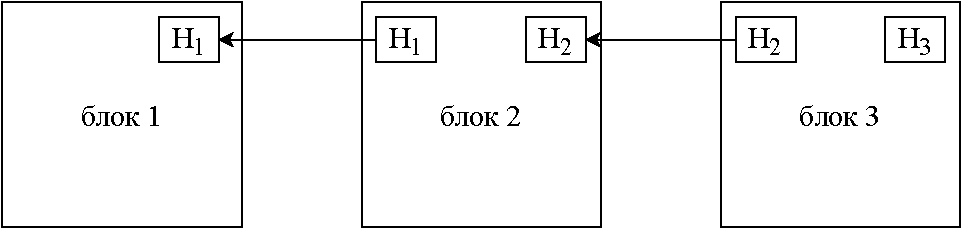
\includegraphics[width=\textwidth]{img/blockchain.pdf}
    \caption{Пример блокчейна}
    \label{fig:blockchain}
\end{figure}

При проверки целостности цепочки выполняются следующие действия:
\begin{enumerate}
    \item Высчитывается хэш от содержимого первого блока и сравнивается со значением хэша, записанным при добавлении данного блока в цепочку. Если значения не совпадают, то констатируется факт наружения целостности.
    \item Для очередного блока вычисляется значение хэша от его содержимого и хэша предыдущего блока. Вычисленное значение сравнивается со значением хэша, записанным при добавлении блока. При несовпадении констатируется факт наружения целостности.
\end{enumerate}

При изменении последнего блока достаточно пересчитать и перезаписать значения хэша только для него. Однако при изменении хэша блока, не являющегося последним, потребуется пересчитать значение хэша всех последующих блоков, что в некоторых системах может потребовать больших вычислительных затрат.

\subsubsection{Дерево и ориентированный ациклический граф Меркла}

Дерево Меркла\cite{merkle} --- двоичное дерево, в листовые вершины которого помещены хеши от блоков данных, а внутренние вершины содержат хеши от сложения значений в дочерних вершинах. В общем случае операция сложения --- произвольная функция от 2 аргументов \textit{f(x, y)}, которая может быть несимметричной (например, конкатенация строк). Корневой узел дерева содержит хеш от всего набора данных, то есть такое дерево является однонаправленной хеш-функцией.

Пример дерева меркла можно увидеть на рисунке \ref{fig:mtree}.

\begin{figure}[hbtp]
    \centering
    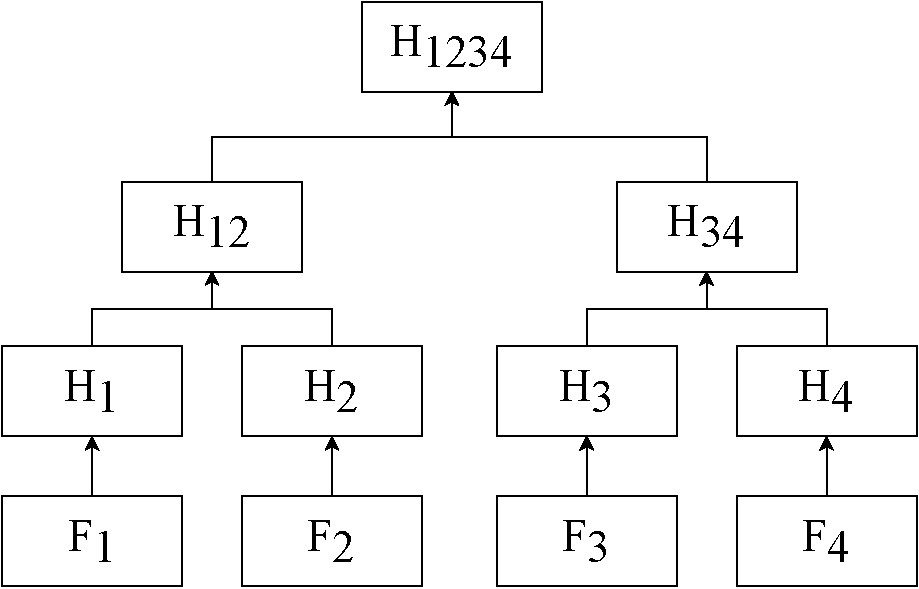
\includegraphics[width=\textwidth]{img/merkletree.pdf}
    \caption{Пример дерева Меркла}
    \label{fig:mtree}
\end{figure}

Применения дерева Меркла:
\begin{itemize}
    \item[---] Хранение транзакций в блокчейне криптовалют (например, в Bitcoin; позволяет получить значение хэша всех транзакций в блоке, а также эффективно верифицировать транзакции).
    \item[---] Для множества значений в среде с ограничением по памяти. В среде хранится только корень дерева. Для проверки принадлежности элемента множеству вместе с элементом требуется передать доказательство Меркла --- значения всех хэшей, с которыми суммируется хэш проверяемого элемента на пути из листа в корень.
\end{itemize}

Ориентированный ациклический граф Меркла\cite{merkledag} --- структура данных, представляющая собой граф, строящийся по следующим правилам:
\begin{enumerate}
    \item Все вершины графа, степень полуисхода\cite{graphs} которых равна 0, представляют хэши данных.
    \item Вычисление значений остальных вершин графа делается в порядке, обратном топологической сортировке\cite{topsort}. Хэшом очередной вершины будет значения хэша от суммы вершин, в которые есть дуга из рассматриваемой вершины.
\end{enumerate}

%
Данная структура данных используется в системе версионного контроля Git\cite{git}.

\subsection{Существующие решения}

В данном подразделе будут описаны существующие системы, решающих задачу обеспечения защиты от неправомерного доступа.

\subsubsection{PASIS}

\label{par:pasis}

PASIS\cite{pasis} --- распределенное хранилище данных, реализующее метод хранения, защищающий от ошибок, связанных с подменой данных определенными узлами системы, называемыми византийскими. Узлы хранилища хранят данные фрагментами и версионируют информацию. Клиенты читают и пишут фрагменты данных.

Клиент пишет данные по фрагментам на \textit{N} узлов хранилища. При чтении данных клиент обращается к \textit{m} узлам, которые являются подмножеством узлов, на которые происходила запись, и проверяет валидность полученных фрагментов. Процесс чтения может быть выполнен в несколько итераций, если в результате валидации будет выявлена ошибка. Процесс чтения считается завершенным, если получено \textit{m} верных фрагментов. Примечательно то, что каждый отдельный фрагмент не несет в себе информации, исходные данные можно восстановить только по \textit{m} и большему числу фрагментам.

Данные восстанавливаются из фрагментов с помощью стирающих кодов\cite{erasurecode} и проверяются с помощью кросс чексумм. Кросс чексумма --- конкатенация хэшей всех \textit{N} записываемых фрагментов. После восстановления данных в наличии у читателя имеется все \textit{N} фрагментов, для которых можно рассчитать хэш-сумму и проверить подлинность данных.

Таким образом использование данной системы позволяет защититься от неправомерного удаления данных с части узлов хранилища с возможностью восстановления данных, а также защититься от неправомерного изменения данных.

\subsubsection{Криптографические файловые системы}

TCFS\cite{tcfs}, NCryptFS\cite{ncryptfs} --- примеры криптографических файловых систем. В отличие от обычных файловых систем, данные системы имеют дополнительный слой между виртуальной файловой системой и драйвером файловой системы, который шифрует данные. При такой реализации работа слоя шифрования данных будет прозрачна для пользователя, потому что пользователь работает с виртуальной файловой системой.

TCFS использует стандартные для файловых систем способы подключения в ОС \texttt{Linux}: системные вызовы \texttt{mount}, \texttt{ioctl} \cite{linux}. При работе в пределах смонтированной файловой системы все операции записи и чтения проходят через слой шифрования, поэтому данные записываются на устройство только в зашифрованном виде.

NCryptFS обладает похожим принципом работы, однако подключается с помощью собственной команды \texttt{attach}, не используя стандартные методы, и имеет возможность создания пространства имен для управления правами групп пользователей на доступ к определенным директориям, а также содержит средства авторизации.

Описанные системы решают задачу неправомерного чтения. При случайной записи данных на устройство будет нарушена их целостность, проверка целостности возлагается на приложения, использующие данные файловые системы, но так как данные хранятся в зашифрованном виде, целостность исходных данных может быть нарушена более значительно. Возможности восстановления данных нет.

\subsubsection{OceanStore}
\label{par:ocean}

OceanStore\cite{ocean} --- безопасная распределенная read-only файловая система.

Данное хранилище хранит данные в одноранговой сети, где узлы соединены между собой по принципу точка-точка. Преимуществом данного хранилища является хранение данных по фрагментам с использованием стирающих кодов. Данный подход, как уже было показано в \ref{par:pasis}, позволяет получать исходные данные, записанные как \textit{N} фрагментов, из любых \textit{m} фрагментов, где $m < N$.

В данном хранилище используется понятие самопроверяющихся данных\cite{selfverify}: данные адресуются по идентификатору GUID, который является хэшом от содержимого. Данный хэш считается из дерева Меркла, изображенного на рисунке \ref{fig:ocean}. Каждый фрагмент помимо самих данных содержит в себе также доказательство Меркла. При восстановлении данных проверяется каждый фрагмент по отдельности (с помощью доказательства Меркла), а также все данные целиком. Порядок действий можно описать следующим образом:
\begin{enumerate}
    \item Получить \textit{m} фрагментов, проверив у каждого доказательство Меркла.
    \item Восстановить \textit{N} фрагментов с использованием стирающих кодов.
    \item Восстановить данные из \textit{N} фрагментов. % (более сложная операция, чем конкатенация строк в общем случае)
    \item Построить дерево Меркла и убедиться в равенстве корня дерева и GUID.
\end{enumerate}

\begin{figure}[hbtp]
    \centering
    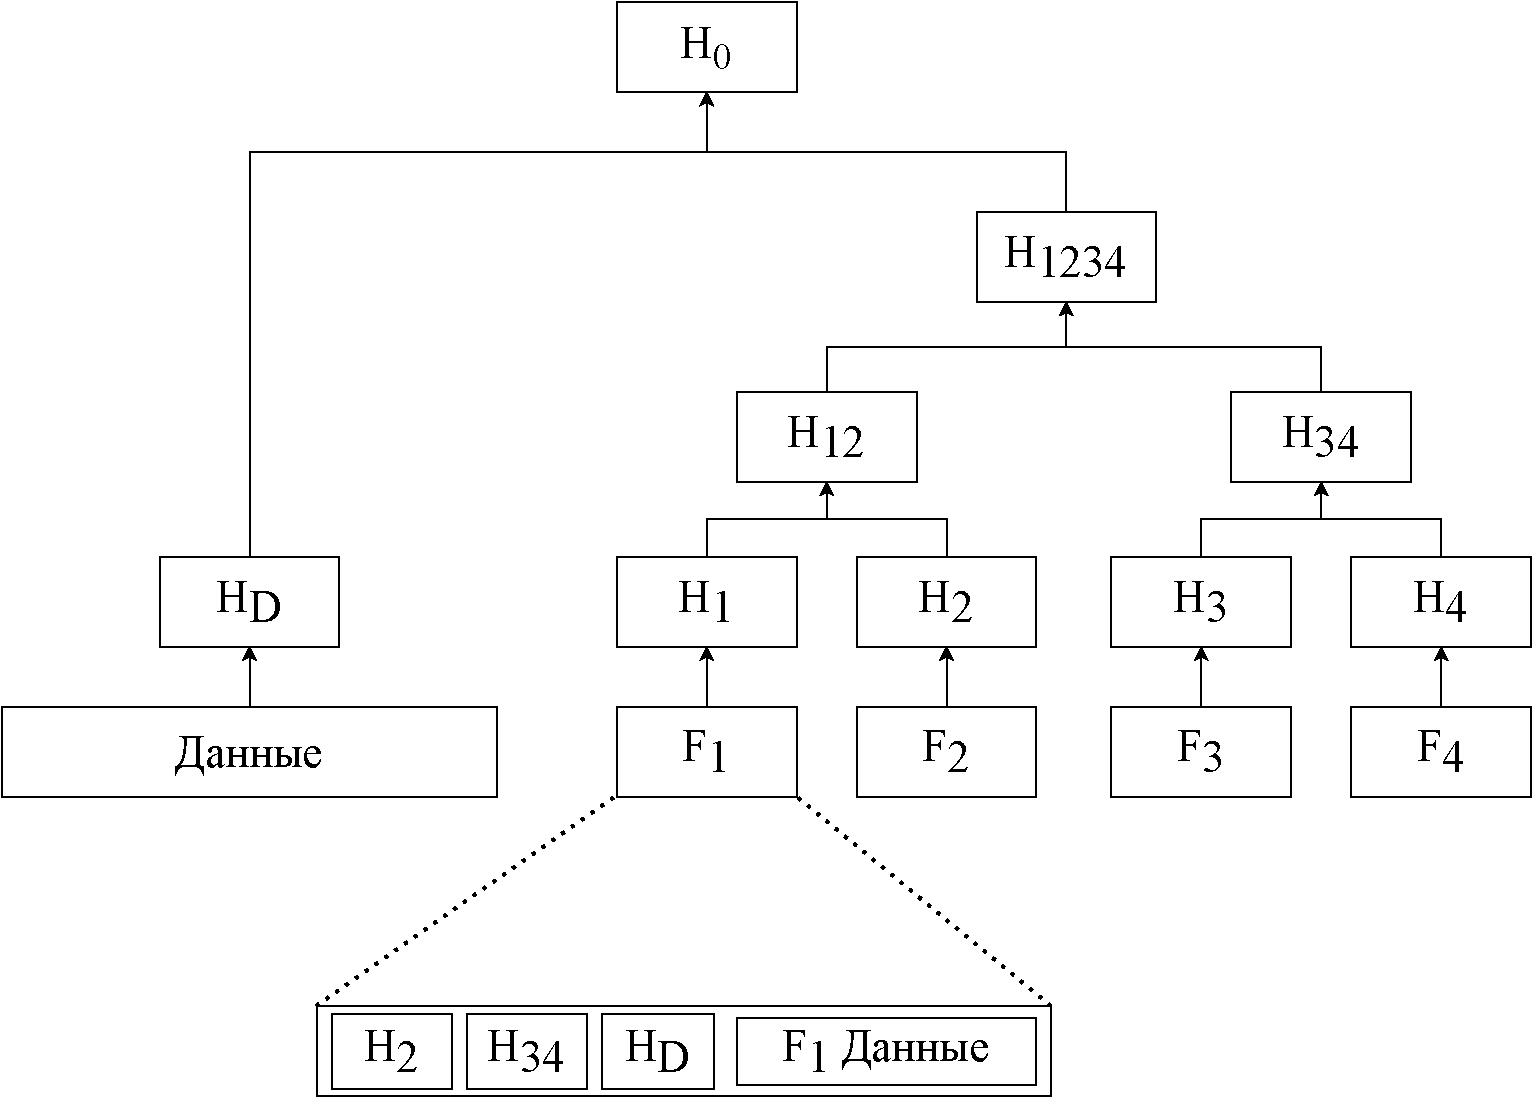
\includegraphics[width=\textwidth]{img/ocean.pdf}
    \caption{Пример дерева Меркла и фрагментов для OceanStore.}
    \label{fig:mtree}
\end{figure}

Данная система считается read-only, потому что изменение данных без изменения идентификатора невозможно, так как идентификатор создается на базе содержимого. Таким образом, например, для обновления версии каких-то данных, старая версия остается неизменной, при этом появляется новая версия с новы содержимым и GUID.

Данное хранилище, несмотря на внутренее устройство, поддерживает возможность иерархической структуры данных. Для этого требуется в некоторых объектах, которые не являются листьями дерева иерархии данных, хранить хэши дочерних вершин. GUID корня иерархической структуры известен.

На примере иерархической структуры видна сложность изменения данных: изменение элемента дерева приводит к необходимости изменения (замены на новый элемент) всех вершин-предков.

Также как и хранилище из раздела \ref{par:pasis}, данная система защищена от частичного удаления данных, обладает возможностью восстановления, а также защищена от неправомерного изменения данных.

\subsubsection{Git}

Git\cite{git} --- система контроля версий. Данная система не решает задачу защиты от неправомерного доступа непосредественно, однако делает это косвенно: при нарушении целостности данных система перестанет работать, что будет являться доказательством неправомерного доступа. Внутреннее представление Git --- хранилище, адресующее по содержанию. Это означает, что файлы, которыми оперирует Git в рамках системной файловой системы, хранятся в виде ассоциативного массива, доступ в котором осуществляется по ключу. Данная система называется Object Store. В качестве ключа файла выступает хэш от его содержимого, подобно GUID в \ref{par:ocean}.

Иерархическую структуру файлов Git поддерживает в виде ориентированного ациклического графа Меркла за счет наличия 3 основных типов объектов:
\begin{enumerate}
    \item blob --- содержит информацию о конкретной версии файла. В ациклическом графе Меркла файлы этого типа всегда обладают нулевой степенью полуисхода, то есть их хэш составлен на основе содержимого файла. Этим же хэшом данные файлы адресуются в упомянутом выше ассоциативном массиве.
    \item tree --- содержит информацию о конкретной версии директории. Данный объект "содержит в себе" объекты (больше 0), которые могут быть типа blob или tree. Он обладает отличной от обычной функцией суммирования: вместо простой конкатенации хэшей вершин, в которые ведут дуги, в функции суммирования также фигурируют имена файлов дочерних вершин (реальные имена, не хэши), а также режимы доступа к данным файлам.
    \item commit --- содержит информацию о коммите --- фиксированном состоянии системы. commit обладает единичной степенью полуисхода и единственная его дуга ведет в объект типа tree, соотвествующей корневой директории репозитория. Объект типа commit хранит информацию об авторе изменений, связанных с фиксацией, об имени, хэше и режиме доступа корневой директории и \textbf{информацию о хэше родительского коммита} --- то есть предыдущей зафиксированной версии. Адресуется коммит значением хэш функции от его содержимого. Схема, по которой описанный коммит связан с предыдущим в точности соответствует схеме работы с блокчейном.
\end{enumerate}

На рисунке \ref{fig:git1} схематично представлен пример графа для 3 основных типов объектов.

\begin{figure}[hbtp]
    \centering
    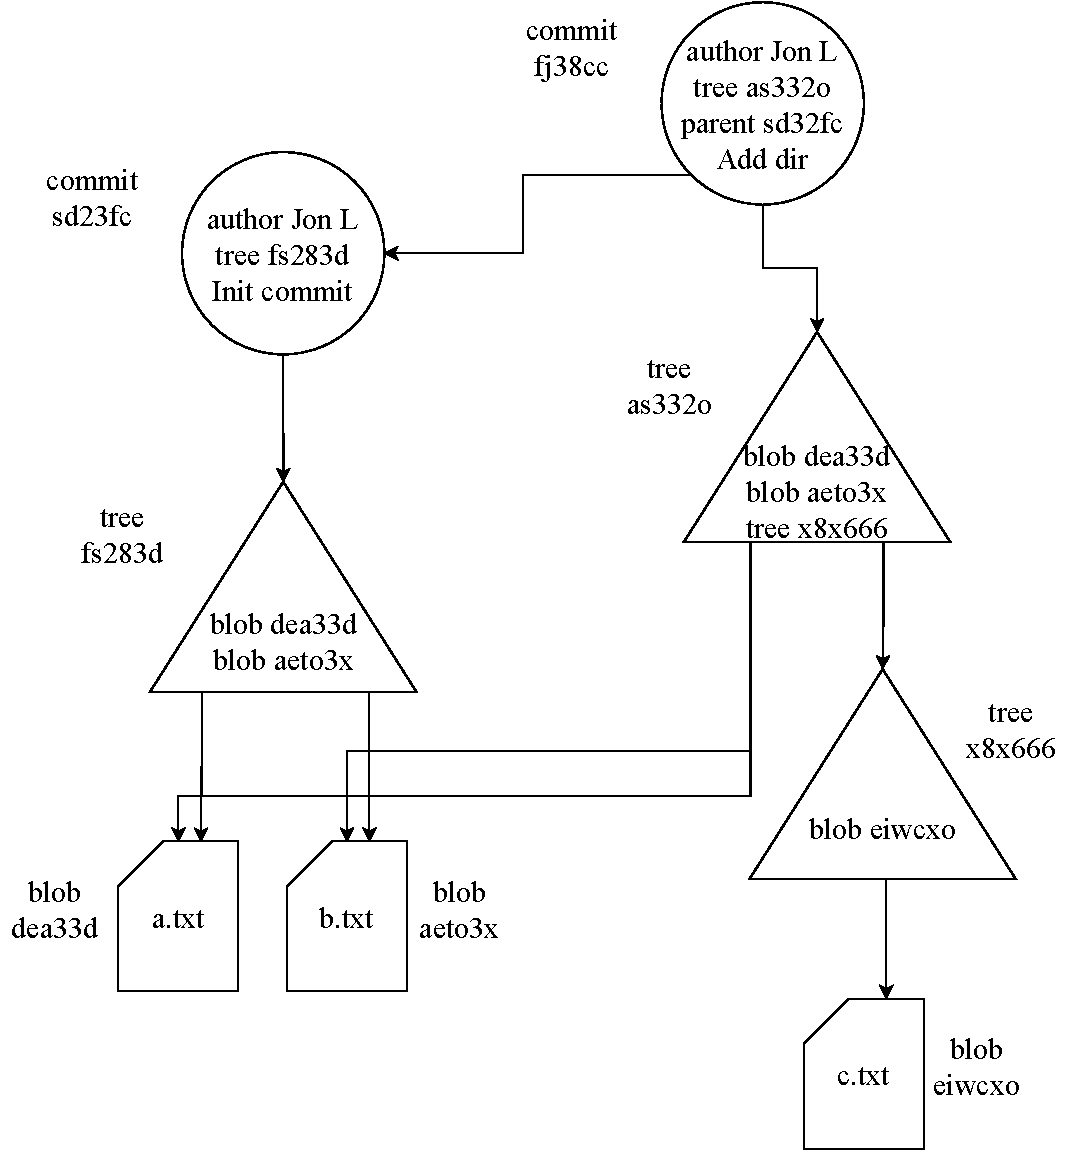
\includegraphics[width=\textwidth]{./img/git-mdag.pdf}
    \caption{Пример графа Меркла для 3 основных типов объектов}
    \label{fig:git1}
\end{figure}

Изменение внутренней структуры в процессе изменения данных происходит:
\begin{enumerate}
    \item Изначально Git не будет учитывать изменения в рабочей директории, то есть при изменении файла у системы будет иметься копия файла из рабочей директории, которая не будет изменена.
    \item Чтобы система учла изменения, требуется добавить измененные файлы в индекс. Данное действие приведет к изменению с точки зрения внешнего интерфейса, с точки зрения внутренней системы это приведет к созданию нового объекта типа blob в Object Store, а также виртуального объекта типа tree (данный объект не будет виден в Object Store на этом этапе). Возможное состояние системы на этом этапе изображено на рисунке \ref{fig:git2}.
    \item При фиксации изменений виртуальный объект типа tree, соответствующий корню рабочей директории для новых версий файлов, добавленных в индекс, становится реальным, то есть создается объект в Object Store, а также создается объект типа commit, который ссылается (содержит хэш в качестве значения) на вновь созданный объект типа tree. Возможное состояние после всех проделанных действий изображено на рисунке \ref{fig:git3}.
\end{enumerate}

\begin{figure}[hbtp]
    \centering
    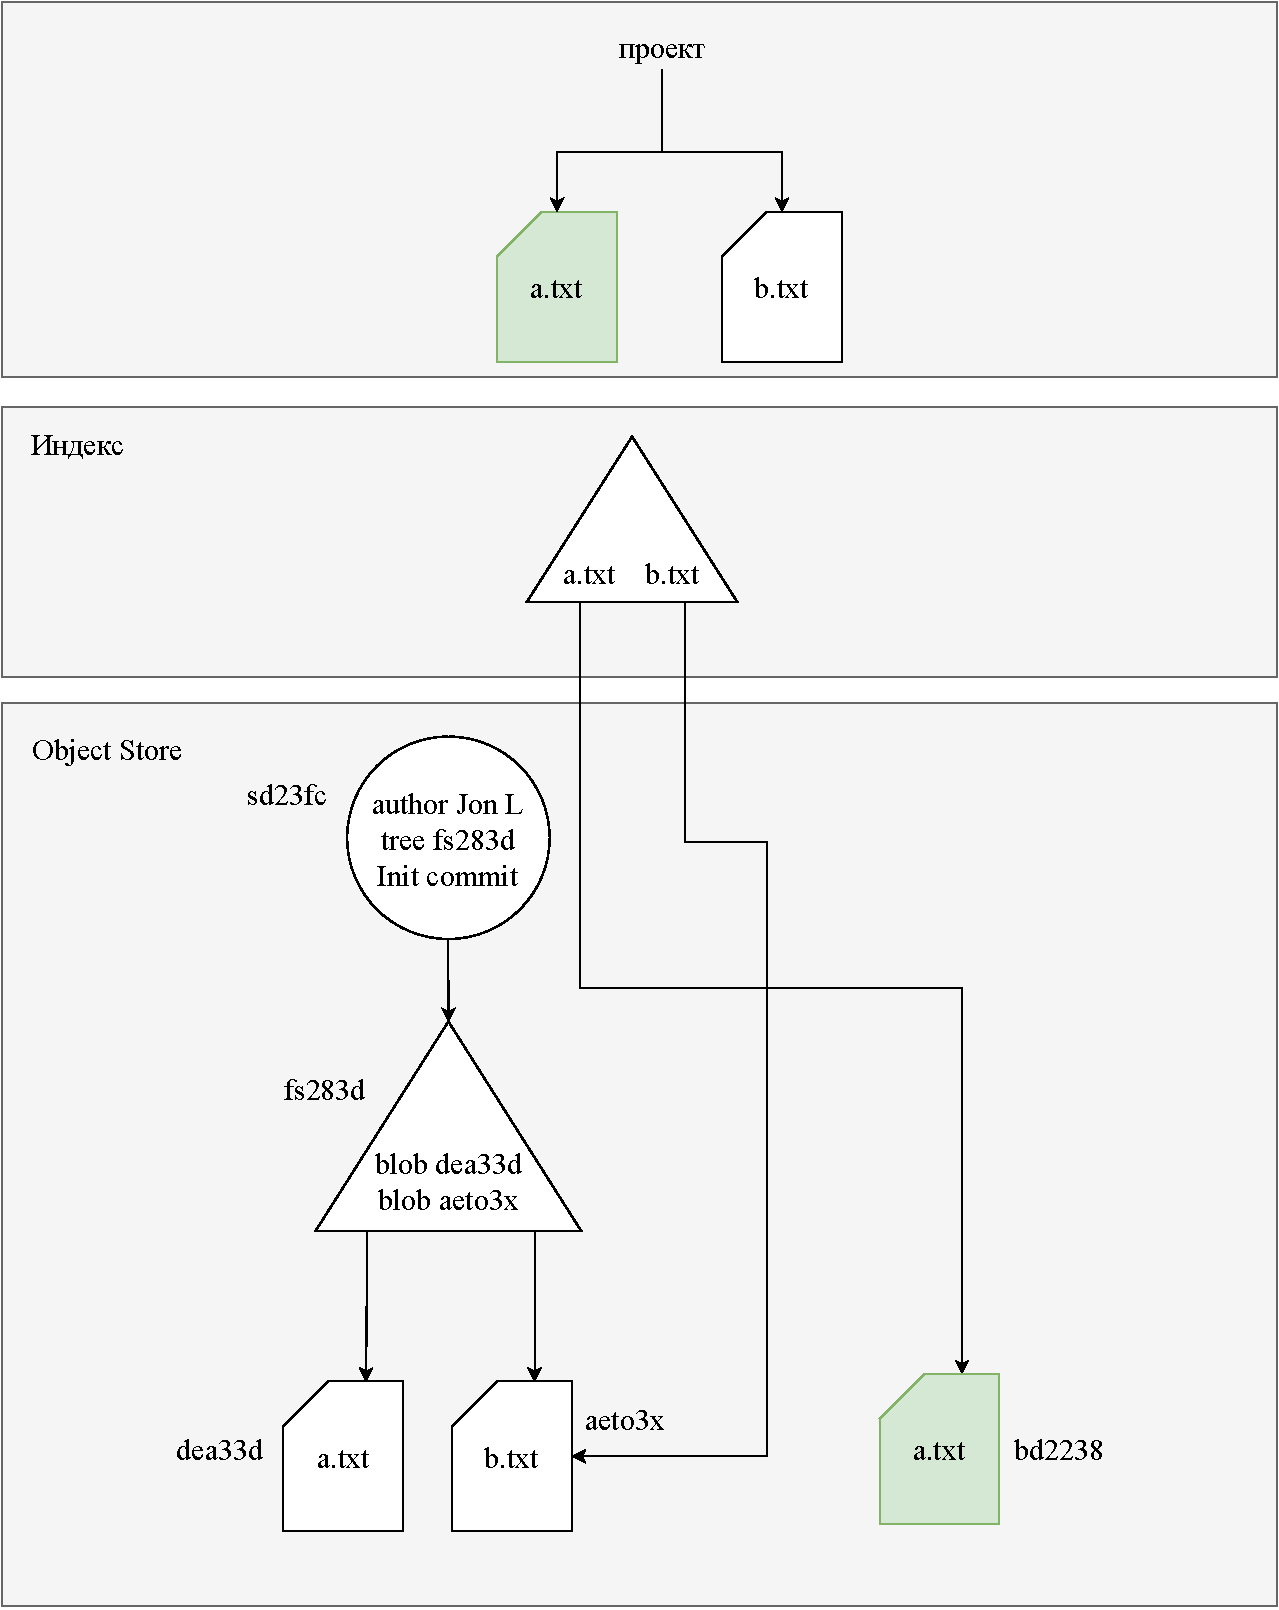
\includegraphics[width=\textwidth]{./img/git-add.pdf}
    \caption{Возможное состояние системы контроля версий Git при добавлении нового файла в индекс.}
    \label{fig:git2}
\end{figure}

\begin{figure}[hbtp]
    \centering
    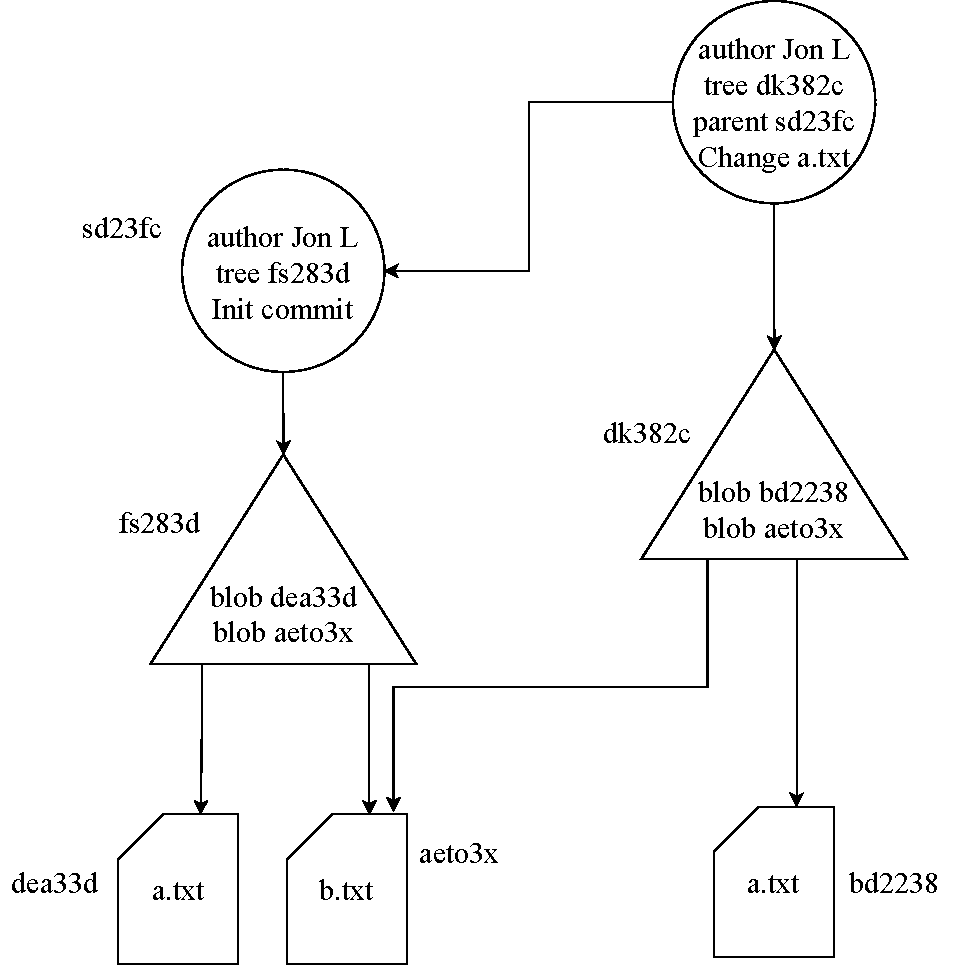
\includegraphics[width=\textwidth]{./img/git-commit.pdf}
    \caption{Возможное состояние системы контроля версий Git после фиксирования изменений.}
    \label{fig:git3}
\end{figure}

Неправомерный доступ подразумевает возможность доступа на запись к внутренней структуре, изменения в которой происходят исключительно засчет добавления новых объектов.

Возможно 3 варианта:
\begin{enumerate}
    \item Изменение данных в рамках объекта. Имя файла в системе Git --- его хэш и любое изменение содержимого приведет к несовпадению рассчитываемого хэша и имени файла, что приведет к ошибке и обнаружению нарушения в данных.
    \item Удаление объекта. Такая атака будет обнаружена в момент, когда произойдет попытка обращения к удаленному файлу. Он не будет найден в Object Store и будет ошибка.
    \item Добавление объекта. Добавление объекта не будет обнаружено, однако и данные, добавленные с новым объектом не будут использованы ввиду того, что никакой другой объект не будет ссылаться на вновь созданный. Если добавить коммит в конце цепочки, то появляется возможность посчитать хэш вместе с хэшем предыдущего commit объекта, однако подобный формат работы похож на стандартный и может быть осуществлен извне.
\end{enumerate}

\clearpage

\subsubsection{Bitcoin}

Bitcoin\cite{bitcoin} --- одноранговая децентрализованная электронная денежная система.

Для данной системы недопустимы сценарии, при которых данные теряются и приводится только доказательство неправомерного доступа к данным. Ввиду того, что данная система является распределенной, у нее нет единого состояния, что усложняет получение неправомерного доступа к данным и их изменение или повреждение без возможности восстановления.

Транзакция --- операция передачи биткойнов с одного адреса на другой. Транзакция осуществляется следующим образом:

\begin{enumerate}
    \item Владелец биткойн-адреса (который связан с публичным ключом) использует любую совершенную транзакцию, в которой адресом назначения является данный адрес.
    \item Создается новая транзакция, которая содержит информацию о наборе адресов и соответсвующем количестве биткоинов, которые требуется перевести в рамках транзакции.
    \item Данная транзакция подписывается приватным ключом владельца кошелька, с которого происходит передача биткоинов.
\end{enumerate}

Таким образом невозможность неправомерного изменения транзакции обеспечивается за счет PKI\cite{pki}.

Транзакция является составным элементом блока. Блок --- составленный по определенным правилам набор транзакций.

Блок имеет определенную структуру, в которую входят:
\begin{itemize}
    \item[---] магическое число;
    \item[---] размер блока;
    \item[---] заголовок блока;
    \item[---] счетчик транзакций;
    \item[---] набор транзакций.
\end{itemize}

Заголовок блока состоит из следующих полей:
\begin{itemize}
    \item[---] версия блока;
    \item[---] хэш заголовка предыдущего блока;
    \item[---] хэш корня дерева Меркла, составленного из транзакций, входящих в данный блок;
    \item[---] текущее время;
    \item[---] целевое значение хэша, ниже которого должен быть хэш от заголовка;
    \item[---] число \textit{Nonce}, которое подбирается таким образом, чтобы хэш от заголовка был меньше целевого значения.
\end{itemize}

Блоки образуют блокчейн --- в заголовке очередного блока содержится хэш предыдущего блока, с помощью которого блоки собираются в цепь. Из одного блока может исходить несколько других блоков, которые содержат первый, как предшествующий. Действующей цепочкой считается наиболее длинная. В этом смысл концепции, называемой proof-of-work: большинство пользователей берут наиболее длинную цепочку блоков и коллективно пытаются подобрать требуемое значение \textit{Nonce}, которое бы удовлетворяло условию целевого значения, тем самым концентруя вычислительные мощности и не давая другим цепочкам стать длиннее текущей. Наиболее быстро будет рассчитываться та цепочка, для расчета которой используется наибольшее количество мощностей.

Сложность расчета значений \textit{Nonce} контролируется за счет изменения целевого значения хэша. Можно дать вероятностную оценку сложности вычисления нужного значения хэша в количестве попыток, исходя из следующих условий:
\begin{itemize}
    \item[---] значение хэш функции является случайным значением;
    \item[---] число нулей в бинарном представлении целевого значения равняется числу $M$.
\end{itemize}

Тогда вероятность появления такого значения хэша, которое будет меньше целевого значения, равна вероятности выпадения $M$ первых нулей при расчете хэша и рассчитывается по формуле \ref{eq:pnce}.

\begin{equation}
    \label{eq:pnce}
    P = \frac{1}{2^M}
\end{equation}

С учетом независимости расчетов для различных $Nonce$ и формулы \ref{eq:pnce}, можно рассчитать количество попыток, требуемых совершить в среднем для получения одного удовлетворяющего числа по формуле \ref{eq:enonce}.

\begin{equation}
    \label{eq:enonce}
    N = \frac{1}{\frac{1}{2^M}} = 2^M
\end{equation}

Наиболее известный способ атаки на системы, работающие по концепции proof-of-work --- атака 51\%. Суть атаки заключается в том, что атакующий владеет большинством вычислительных мощностей и делает следующие действия:
\begin{enumerate}
    \item Сделать блок, который будет содержать некоторую транзакцию $T_1$.
    \item Дождаться, пока система, на счет которой мы перевели биткоины, будет считать транзакцию $T_1$ завершившейся.
    \item Взять блок, предшествующий блоку из пункта 1, и начать делать новую цепочку без транзакции $T_1$ до тех пор, пока она не станет действующей.
\end{enumerate}

Такая атака позволяет неправомерно изменить данные.

\subsubsection{Выводы}

Сравнение рассмотренных методов хранения данных с возможностью защиты от неправомерного доступа можно увидеть в таблице \ref{tab:res}. Обозначения:
\begin{itemize}
    \item[---] НД --- неправомерное действие;
    \item[---] КФС --- криптографические файловые системы;
    \item[---] У --- удаление;
    \item[---] И --- изменение;
    \item[---] ЧУ --- частичное удаление;
    \item[---] ЧИ --- частичное изменение.
\end{itemize}

Полученные результаты можно свести к следующему:
\begin{itemize}
    \item[---] Защита от чтения возможна в системе, в которой определенная группа людей обладает некоторым уникальным знанием (ключ в КФС).
    \item[---] Восстановление данных после частичного изменения или удаления возможно в распределенных системах, использующих стирающий код, в связи с тем, что фрагменты хранятся в разных местах и допускается неправомерный доступ в части мест.
    \item[---] Исключает возможность полного неправомерного изменения только Bitcoin, потому что во всех рассмотренных системах количество узлов, в которых хранятся данные, конечно и задано наперед (хоть и в теории может быть очень велико), в то время как в Bitcoin все узлы системы содержат одно состояние.
    \item[---] Возможностью доказательства неправомерного изменения обладают все системы кроме КФС, используя для этого контрольные суммы и хэши. Однако также как в случае удаления, в локальной системе без шифрования нарушитель может восстановить целостность цепочки блоков при изменении внутреннего состояния Git.
    \item[---] Возможностью доказательства неправомерного удаления обладают 2 системы, в основе которых лежит блокчейн. Однако если данные не шифруются никаким образом, то в случае с Git человек, нарушающий права, способен повторить действия самой системы, и произвести изменения, поддержав целостность цепочки блоков.
\end{itemize}

\begin{table}[h]
    \begin{center}
        \label{tab:res}
        \caption{Методы хранения и обеспечиваемая защита.}
        \begin{tabular}{|c|c|c|c|c|c|}
            \hline
            \bfseries НД & \bfseries PASIS & \bfseries КФС & \bfseries OceanStore & \bfseries Git & \bfseries Bitcoin  \\
            \hline
            чтение (исключение) & - & + & - & - & - \\ \hline
            ЧУ или ЧИ (восстановление) & + & - & + & - & - \\ \hline
            изменение (исключение) & - & - & - & - & + \\ \hline
            изменение (доказательство) & + & - & + & +/- & + \\ \hline
            удаление (доказательство) & - & - & - & +/- & + \\ \hline
        \end{tabular}
    \end{center}
\end{table}

\clearpage

\subsection{Архитектура СУБД ClickHouse}

В данном разделе будет рассмотрена архитектура СУБД ClickHouse.

\subsubsection{Основные концепции}

ClickHouse --- полноценная колоночная СУБД. Данные хранятся в колонках, а в процессе обработки - в массивах. По возможности операции выполняются на массивах, а не на индивидуальных значениях. Это называется <<векторизованное выполнения запросов>>, и помогает снизить стоимость фактической обработки данных.

Для представления фрагментов столбцов в памяти используется интерфейс \texttt{IColumn}. Интерфейс предоставляет вспомогательные методы для реализации различных реляционных операторов. Почти все операции иммутабельные: они не изменяют оригинальных колонок, а создают новую с измененными значениями.

Различные реализации \texttt{IColumn} (например, \texttt{ColumnUInt8} или \texttt{ColumnString}) отвечают за распределение данных колонки в памяти. Для колонок целочисленного типа это один смежный массив, такой как \texttt{std::vector}. Для колонок типа String и Array это два вектора: один для всех элементов массивов, располагающихся смежно, второй для хранения смещения до начала каждого массива. Также существует реализация \texttt{ColumnConst}, которая несмотря на то, что хранит только одно значение в памяти, обладает поведением фрагмента колонки.

Можно работать и с индивидуальными значениями. Для представления индивидуальных значений используется Поле (\texttt{Field}). \texttt{Field} --- размеченное объединение \texttt{UInt64}, \texttt{Int64}, \texttt{Float64}, \texttt{String} и \texttt{Array}. \texttt{Field} не несет в себе достаточно информации о конкретном типе данных в таблице (например, \texttt{UInt8}, \texttt{UInt16}, \texttt{UInt32} и \texttt{UInt64} в \texttt{Field} представлены как \texttt{UInt64}).

Различные функции на колонках могут быть реализованы обобщенным, неэффективным путем, используя \texttt{IColumn} методы для извлечения значений \texttt{Field}, или специальным путем, используя знания о внутреннем распределение данных в памяти в конкретной реализации \texttt{IColumn}. Для этого функции приводят \texttt{IColumn} к конкретному типу и работают напрямую с его внутренним представлением.

\texttt{IDataType} отвечает за сериализацию и десериализацию --- чтение и запись фрагментов колонок или индивидуальных значений в бинарном или текстовом формате.  \texttt{IDataType} точно соответствует типам данных в таблицах.

\texttt{IDataType} и \texttt{IColumn} слабо связаны друг с другом. Различные типы данных могут быть представлены в памяти с помощью одной реализации \texttt{IColumn} (например, и \texttt{DataTypeUInt32}, и \texttt{DataTypeDateTime} в памяти представлены как \texttt{ColumnUInt32} или \texttt{ColumnConstUInt32}).

\texttt{IDataType} хранит только метаданные (например, \texttt{DataTypeFixedString} хранит только N --- фиксированный размер строки).

\texttt{Block} это контейнер, который представляет фрагмент таблицы в памяти. Это набор троек --- \texttt{(IColumn, IDataType, имя колонки)}. В процессе выполнения запроса, данные обрабатываются блоками. Если имеется \texttt{Block}, значит имеются данные (в объекте \texttt{IColumn}), информация о типе (в \texttt{IDataType}) и имя колонки. Блоки создаются для всех обработанных фрагментов данных.

\subsubsection{Движок MergeTree}

Основная идея движка MergeTree заключается в том, что данные записываются кусками в своем изначальном виде, а затем данные куски объединяются в фоновом режиме. Данных подход используется для исключения большого количества перезаписи данных для сохранения требуемого порядка элементов.

Таблица состоит из кусков данных, отсортированных по первичному ключу. При вставке в таблицу создаются отдельные куски данных, каждый из которых лексикографически отсортирован по первичному ключу.

Данные, относящиеся к разным партициям, разбиваются на разные куски. В фоновом режиме ClickHouse выполняет слияния (merge) кусков данных для более эффективного хранения. Куски, относящиеся к разным партициям не объединяются. Механизм слияния не гарантирует, что все строки с одинаковым первичным ключом окажутся в одном куске.

Каждый кусок данных логически делится на гранулы. Гранула --- минимальный неделимый набор данных, который ClickHouse считывает при выборке данных. ClickHouse не разбивает строки и значения и гранула всегда содержит целое число строк. Первая строка гранулы помечается значением первичного ключа для этой строки (засечка). Для каждого куска данных ClickHouse создаёт файл с засечками (индексный файл). Для каждого столбца, независимо от того, входит он в первичный ключ или нет, ClickHouse также сохраняет эти же засечки. Засечки используются для поиска данных напрямую в файлах столбцов.

Размер гранул оганичен настройками движка по количеству и байтам. Количество строк в грануле лежит в диапазоне не больше максимально заданного значения, в зависимости от размера строк. Размер гранулы может превышать максимально заданный размер в байтах в том случае, когда размер единственной строки в грануле превышает значение настройки. В этом случае, размер гранулы равен размеру строки.

TODO: написать подробнее про движок

\subsubsection{Специфика выполнения операций над данными в MergeTree}

Здесь надо написать про альтеры и про мержи (слияния).

\subsection{Метод защиты от неправомерного доступа в движке MergeTree}

Здесь надо описать свой метод в 2 моментах

\subsubsection{Хранимые данные и связывание блоков}

\subsubsection{Пересчет хэшей во время изменений и слияний}

\pagebreak